\subsubsubsection{Interaction between entities}

The application contains several interactions among entities that have to be
specified in order to understand well how to approach different problems.

\paragraph{Entering a road} Moving entities enter a road by entering a stretch
that is located at the beginning of the road and that is treadable by their
specific entity type.

\paragraph{Entering a road stretch} Moving entities who want to enter a new
road stretch can do it whenever there is room for them in that stretch. In
particular, a roadway stretch can be trod for at most one vehicle at the same
time.

\paragraph{Zebra crossings} Vehicles which want to enter a road stretch that
has zebra crossings painted on it has to wait for pedestrians or bikes to free
all stretches of that particular crossing.

\paragraph{Changing roadway lane} A vehicle that is on the i-th road stretch
which wants to change lane has to wait until the (i+1)-th stretch in the
wanted direction is free.

\paragraph{Crossroads} Every road that is connected to a crossroads is marked
with a cardinal point (N/E/W/S). The crossroads holds all the logic necessary
for vehicles to follow the yield rules we described in
\ref{sec:pa-domain-problems}.

There could be a situation in which there is a standstill, for example when
four cars want all to go straight in a four-way crossroads. In this case, the
crossroads will make a car yield the right-of-way to another one.

Pedestrians can only walk on the corner of the crossroads, thus passing to the
adjacent piece of road (e.g. a pedestrian that is coming from the ``southern''
side of the western road can only enter the southern street on the ``western''
side).

\paragraph{Entering a building} When a moving entity is in the stretch where
there is the entrance of a building, then it may enter the building.

If the moving entity is a vehicle, it has to wait for all other entities who
are in the intermediate stretches to move away.

\paragraph{Exiting a building} When a moving entity is exiting a building, it
has to check whether there is room for her to move out.

If the entity is a vehicle, it has to yield the right-of-way to upcoming
vehicles and to wait that eventual sidewalks or bicycle path stretches in front
of the building are free too.

\paragraph{Choosing to use a vehicle} An entity $e$ who wants to leave a
building $b_e$ to a destination $d_e$ may randomly decide not to travel by
foot. She can leave only if:

\begin{itemize}
  \item the path from $b_e$ to $d_e$ does not include any destination of other
    people who are leaving from $b$ and viceversa. Otherwise, they would share
    the vehicle if there is enough room;
  \item there is an available vehicle in $b_e$; and
  \item the capacity of the destination building $d_e$ is greater than the sum
    of all vehicles in it and the ones which are arriving to that building.
\end{itemize}

If all of these conditions are met, then:
\begin{itemize}
  \item the entity may exit the building and travel using a vehicle; and
  \item $d_e$ now ``books'' a place for the vehicle driven by $e$.
\end{itemize}

\begin{figure}[H]
  \centering
  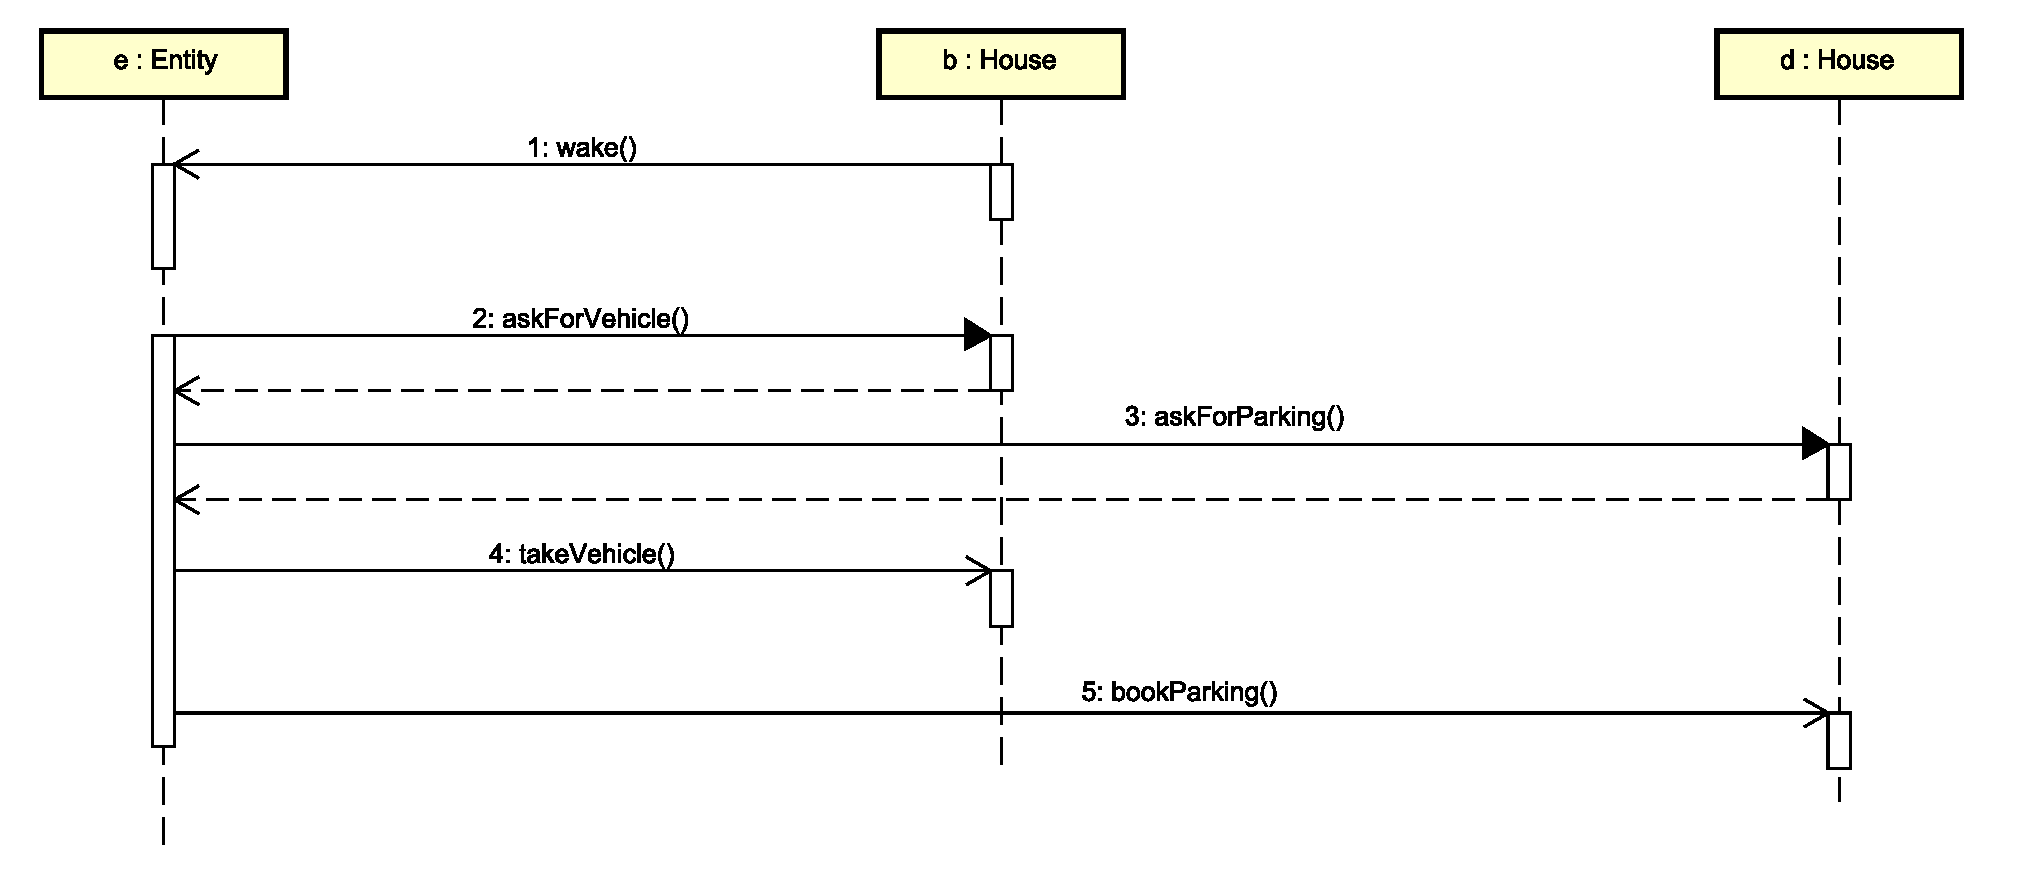
\includegraphics[width=\columnwidth,trim=1 0 0 0,clip]
    {sections/images/solution/going-out-vehicle.eps}
  \caption{Exiting a building with a vehicle}
  \label{fig:app-inter-vehicle}
\end{figure}

\paragraph{Waiting for a bus} A pedestrian may randomly decide to wait for a
bus if she is on a bus stop stretch.

Firstly, she checks whether the buses that stops at that stretch match (even
partially) her path. If at least one of them does, then she wait for a limited
amount of time for a bus to arrive.

If this timeout expires, then she continues travelling by foot to the next
stretch.

\begin{figure}[H]
  \centering
  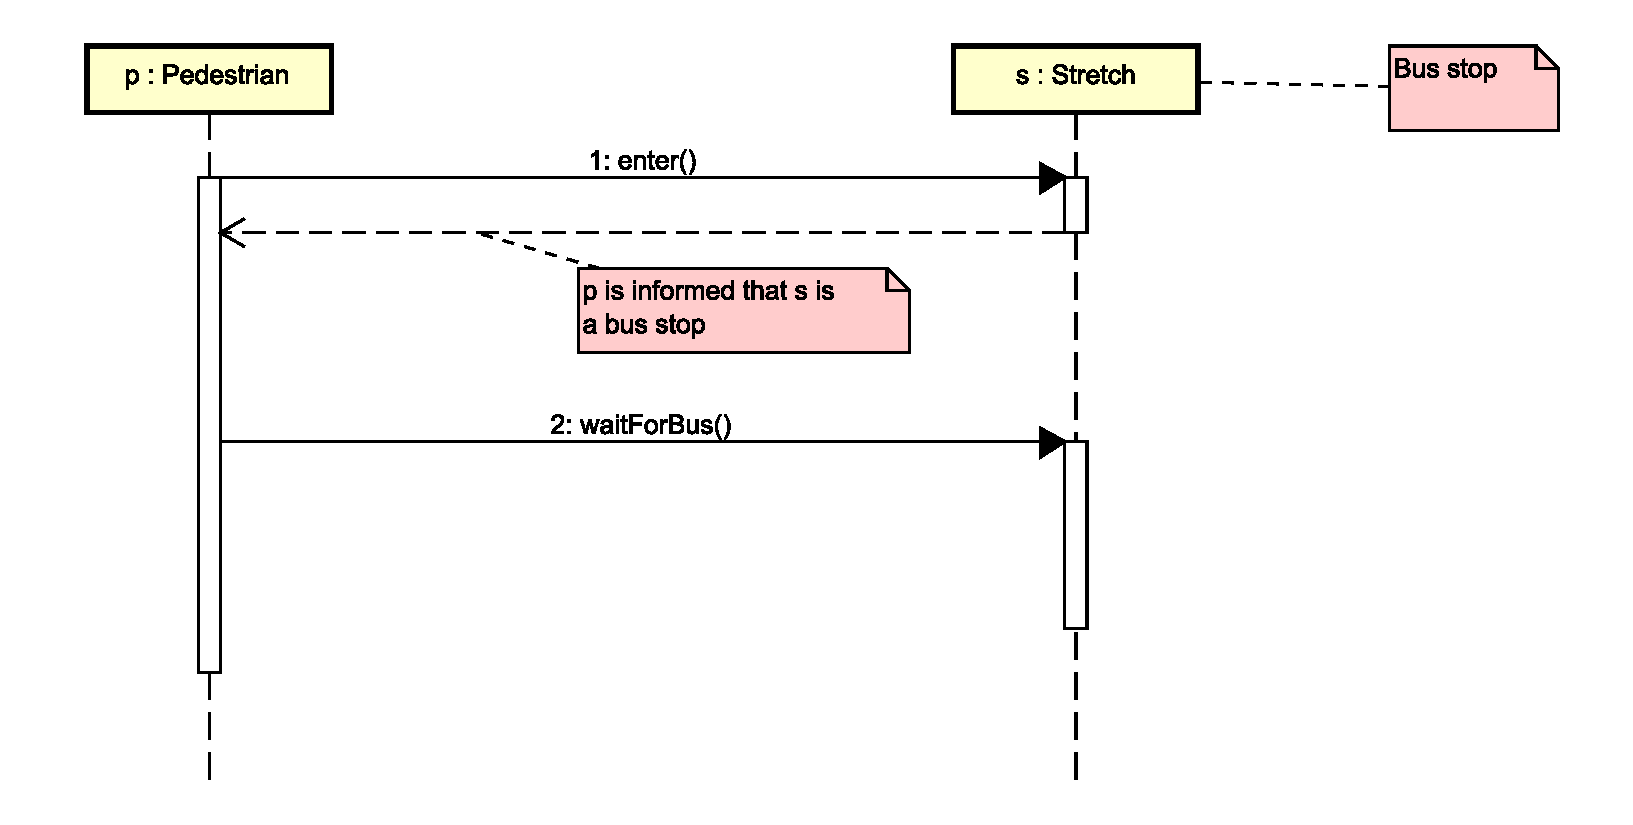
\includegraphics[width=\columnwidth,trim=1 0 2 0,clip]
    {sections/images/solution/bus-waiting.eps}
  \caption{Waiting for a bus}
  \label{fig:app-inter-wait-bus}
\end{figure}

\paragraph{Boarding a bus} When a bus arrives at a bus stop, then a waiting
entity will board it only if:

\begin{itemize}
  \item there is enough room for her; and
  \item this bus shortens the expected route for her.
\end{itemize}

\begin{figure}[H]
  \centering
  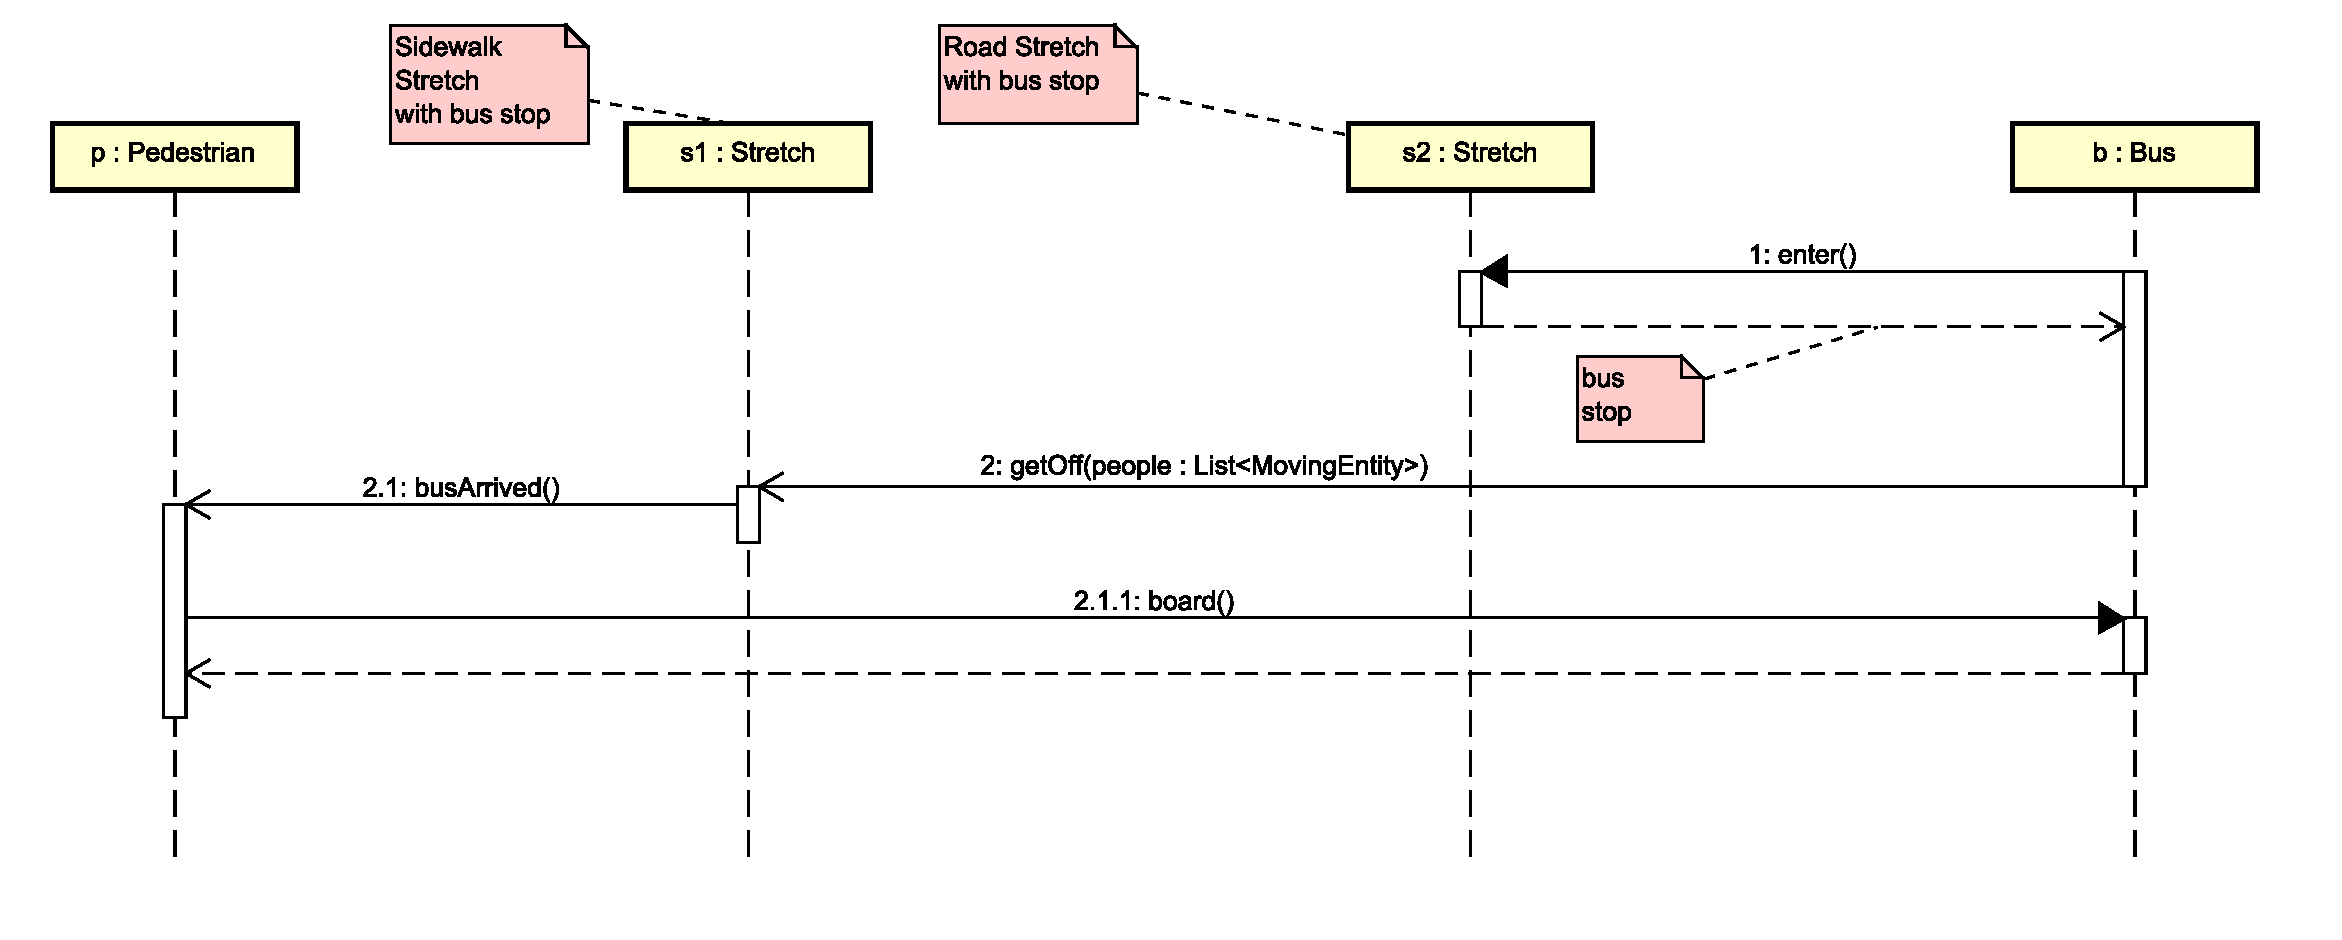
\includegraphics[width=\columnwidth,trim=1 0 0 0,clip]
    {sections/images/solution/bus-boarding.eps}
  \caption{Boarding a bus}
  \label{fig:app-inter-board-bus}
\end{figure}

\paragraph{Getting off a bus} A person $p$ will get off a bus when it reaches
the last stop $s$ such that $s$ belongs to the route of $p$.

\paragraph{Respecting street code} Roads and crossroads will contain all the
necessary logic to make moving entities follow the street rules.

\paragraph{Performing an overtaking} This action is possible only when a
vehicle is able to change lane. It might be triggered by a timeout which
expires when it is waiting too much for entering the next straightaway stretch.

When a vehicle tries to overtake another one, it will always try to return to
the lane where it started the operation before entering the last stretch.
% look for "manovra" translation

% \paragraph{Uber} % Is it a TODO?

